% Use only LaTeX2e, calling the article.cls class and 12-point type.

\documentclass[11pt]{article}

% Users of the {thebibliography} environment or BibTeX should use the
% scicite.sty package, downloadable from *Science* at
% www.sciencemag.org/about/authors/prep/TeX_help/ .
% This package should properly format in-text
% reference calls and reference-list numbers.

%\usepackage{scicite}
\usepackage[numbers, square, sort, compress]{natbib}

% Use times if you have the font installed; otherwise, comment out the
% following line.

\usepackage{times}
\usepackage{hyperref}
\usepackage{graphicx}
\usepackage{amsmath}
\usepackage[left]{lineno}
\linenumbers
% The preamble here sets up a lot of new/revised commands and
% environments.  It's annoying, but please do *not* try to strip these
% out into a separate .sty file (which could lead to the loss of some
% information when we convert the file to other formats).  Instead, keep
% them in the preamble of your main LaTeX source file.


% The following parameters seem to provide a reasonable page setup.

\topmargin 0.0cm
\oddsidemargin 0.2cm
\textwidth 16cm 
\textheight 21cm
\footskip 1.0cm



% If your reference list includes text notes as well as references,
% include the following line; otherwise, comment it out.

\renewcommand\refname{References and Notes}

% The following lines set up an environment for the last note in the
% reference list, which commonly includes acknowledgments of funding,
% help, etc.  It's intended for users of BibTeX or the {thebibliography}
% environment.  Users who are hand-coding their references at the end
% using a list environment such as {enumerate} can simply add another
% item at the end, and it will be numbered automatically.

\newcounter{lastnote}
\newenvironment{scilastnote}{%
\setcounter{lastnote}{\value{enumiv}}%
\addtocounter{lastnote}{+1}%
\begin{list}
{\arabic{lastnote}.}
{\setlength{\leftmargin}{.22in}}
{\setlength{\labelsep}{.5em}}}
{\end{list}}

\newcommand{\taskrecon}{S1}
\newcommand{\perexptaskrecon}{S2}
\newcommand{\perexpcorrmaps}{S3}

% Include your paper's title here

\title{Towards human SuperEEG} 


% Place the author information here.  Please hand-code the contact
% information and notecalls; do *not* use \footnote commands.  Let the
% author contact information appear immediately below the author names
% as shown.  We would also prefer that you don't change the type-size
% settings shown here.

\author
{Lucy L. W. Owen$^{1}$, Andrew C. Heusser$^{1, 2}$, and Jeremy R. Manning$^{1\ast}$\\\\
$^{1}$Department of Psychological and Brain Sciences, Dartmouth College,\\
Hanover, NH 03755, USA\\
$^{2}$Akili Interactive,\\
Boston, MA 02110, USA}

% Include the date command, but leave its argument blank.

\date{}



%%%%%%%%%%%%%%%%% END OF PREAMBLE %%%%%%%%%%%%%%%%


\begin{document} 

% Double-space the manuscript.

\baselineskip24pt

% Make the title.

\maketitle 

\begin{abstract}
  Human \textit{SuperEEG}\footnote{The term ``SuperEEG'' was coined by
    Robert J. Sawyer in his popular science fiction novel \textit{The
      Terminal Experiment}~\cite{Sawy95}} entails measuring ongoing
  neural activity with perfect precision and at arbitrarily high
  spatiotemporal resolution.  Although true SuperEEG is impossible
  using existing methods, here we present a model-based method for
  \textit{inferring} neural activity at millimeter-scale spatial
  resolutions and millisecond-scale temporal resolutions using
  standard human intracranial recordings.  Our approach assumes that
  different people's brains exhibit similar spatial correlations, and
  that (all else being equal) neural activity at nearby locations will
  tend to be similar.  One can then ask, for an arbitrary individual's
  brain: given recordings from a limited set of locations in that
  individual's brain, along with the observed spatial correlations in
  other people's recordings, what would recordings most likely have
  looked like at \textit{other} locations in that individual's
  brain?\\\\
  \footnotesize{\textbf{Keywords: Electrocorticography (ECoG),
      intracranial electroencephalography (iEEG), local field
      potential (LFP), epilepsy, maximum likelihood estimation,
      Gaussian process regression}}
\end{abstract}

\section*{Introduction}
Modern human brain recording techniques are fraught with
compromise~\citep{SejnEtal14}.  Commonly used approaches include
functional magnetic resonance imaging (fMRI), scalp
electroencephalography (EEG), and magnetoencephalography (MEG).  For
each of these techniques, neuroscientists and electrophysiologists
must choose to optimize spatial resolution at the cost of temporal
resolution (e.g., as in fMRI) or temporal resolution at the cost of
spatial resolution (e.g., as in EEG and MEG).  A less widely used
approach (due to requiring work with neurosurgical patients) is to
record from electrodes implanted directly onto the cortical surface
(electrocorticography; ECoG) or into deep brain structures
(intracranial EEG; iEEG).  However, these intracranial approaches also
require compromise: the high temporal and spatial resolutions of
intracranial recordings comes at the cost of substantially reduced
brain coverage, since safety considerations limit the number of
electrodes one may implant in a given patient's brain.  Further, the
locations of implanted electrodes are determined by clinical, rather
than research, needs.

An increasingly popular approach is to improve the effective spatial
resolution of MEG or scalp EEG data by using a geometric approach
called \textit{beamforming} to solve the biomagnetic or bioelectrical
inverse problem~\cite{Sarv87}.  This approach entails using detailed
brain conductance models (often informed by high spatial resolution
anatomical MRI images) along with the known sensor placements
(localized precisely in 3D space) to reconstruct brain signals
originating from theoretical point sources deep in the brain (and far
from the sensors).  Traditional beamforming approaches must overcome
two obstacles.  First, the inverse problem beamforming seeks to solve
has infinitely many solutions.  Researchers have made traction towards
constraining the solution space by assuming that signal-generating
sources are localized on a regularly spaced grid spanning the brain
and that individual sources are small relative to their distances to
the sensors~\cite{Snyd91, BailEtal01, HillEtal05}.  The second, and in
some ways much more serious, obstacle is that the magnetic fields
produced by external (noise) sources are substantially stronger than
those produced by the neuronal changes being sought (i.e., at deep
structures, as measured by sensors at the scalp).  This means that
obtaining adequate signal quality often requires averaging the
measured responses over tens to hundreds of responses or trials
(e.g., see review by~\cite{HillEtal05}).

Another approach to obtaining high spatial and temporal resolution
neural data has been to collect fMRI and EEG data simultaneously.
Simultaneous fMRI-EEG has the potential to balance the high spatial
resolution of fMRI with the high temporal resolution of scalp EEG,
thereby, in theory, providing the best of both worlds.  In practice,
however, the signal quality of both recordings suffers substantially
when the two techniques are applied simultaneously (e.g., see review
by~\cite{HustEtal12}).  In addition, the experimental designs that are
ideally suited to each technique individually are somewhat at odds.
For example, fMRI experiments typically lock stimulus presentation
events to the regularly spaced image acquisition time (TR), which
maximizes the number of post-stimulus samples.  By contrast, EEG
experiments typically employ jittered stimulus presentation times to
maximize the experimentalist's ability to distinguish electrical brain
activity from external noise sources such as from 60 Hz alternating
current power sources.

The current ``gold standard'' for precisely localizing signals and
sampling at high temporal resolution is to take (ECoG or iEEG)
recordings from implanted electrodes (but from a limited set of
locations in any given brain).  This begs the following question: what
can we infer about the activity exhibited by the rest of a person's
brain, given what we learn from the limited intracranial recordings we
have from their brain and additional recordings taken from
\textit{other} people's brains?  Here we develop an approach, which we
call \textit{SuperEEG}, based on Gaussian process
regression~\cite{Rasm06}.  SuperEEG entails using data from multiple
people to estimate activity patterns at arbitrary locations in each
person's brain (i.e., independent of their electrode placements).  We
test SuperEEG approach using two large datasets of intracranial
recordings~\cite{SedeEtal03, SedeEtal07a, SedeEtal07b, MannEtal11,
  MannEtal12, EzzyEtal17, HoraEtal17, KragEtal17, KuceEtal17,
  LinEtal17, SoloEtal18, WeidEtal18, EzzyEtal18, KuceEtal18}.  We show
that the SuperEEG algorithm recovers signals well from electrodes that
were held out of the training dataset.  We also examine the factors
that influence how accurately activity may be estimated (recovered),
which may have important implications for electrode design and
placement in neurosurgical applications.

\section*{Approach}
The SuperEEG approach to inferring high temporal resolution full-brain
activity patterns is outlined and summarized in
Figure~\ref{fig:methods}. We describe (in this section) and evaluate
(in \textit{Results}) our approach using a two large previously
collected dataset comprising multi-session intracranial recordings.
Dataset 1 comprises multi-session recordings taken from 6876
electrodes implanted in the brains of 88 epilepsy
patients~\cite{SedeEtal03, SedeEtal07a, SedeEtal07b, MannEtal11,
  MannEtal12}.  Each recording session lasted from XXX--XXX hours, and
includes data recorded roughly from when the patients woke up each
morning, to before they went to sleep at the end of each day.  In
addition to typical bed-ridden hospital patient activities (e.g.,
lying in bed, reading, watching television, using personal electronic
devices, listening to music, visiting with family and friends, etc.),
the patients also performed a variety of experimental cognitive tasks
throughout their day (primarily list-learning memory tasks).  For the
purposes of the Dataset 1 analyses presented here, we aggregated all
data across each recording session, ignoring the particular activities
or tasks the patients were performing at any given moment.  We used
Dataset 1 to develop and debug our main SuperEEG approach, and to
examine the extent to which SuperEEG might be able to generate
task-general predictions.  Dataset 2 comprised multi-session
recordings from XXX electrodes implanted in the brains of XXX epilepsy
patients~\citep{EzzyEtal17, HoraEtal17, KragEtal17, KuceEtal17,
  LinEtal17, SoloEtal18, WeidEtal18, EzzyEtal18, KuceEtal18}.  Whereas
Dataset 1 included recordings taken during a wide variety of
behaviors, Dataset 2 included recordings taken as each patient
performed each of two memory tasks: a random word list free recall
task and a categorized word list free recall task.  We used Dataset 2
to further examine the ability of SuperEEG to generalize its
predictions within versus across tasks.

\begin{figure}
  \centering
  \includegraphics[width=\textwidth]{figs/methods}
  \caption{\textbf{Methods overview.}  \textbf{A.  Electrode
      locations.}  Each dot reflects the location of a single
    electrode in dataset 1, colored according to 7 factor labels (see
    Panel D for details). One patient's electrode locations are
    highlighted in black and the to-be-reconstructed recording
    location is highlighted in red. \textbf{B. Radial basis function
      (RBF).}  Each electrode contributed by the patient (black)
    weights on the full set of locations under consideration (all dots
    in Panel A, defined as $\bar{R}$ in the text).  The weights fall
    off with positional distance (in MNI space) according to an RBF.
    \textbf{C. Per-patient correlation matrices.}  After computing the
    pairwise correlations between the recordings from each patient's
    electrodes, we use RBF-weighted averages to estimate correlations
    between all locations in $\bar{R}$.  We obtain an estimated
    full-brain correlation matrix using each patient's
    data. \textbf{D.  Combined correlation matrix.}  We estimate a
    single full-brain correlation matrix by averaging the
    patient-specific correlation matrices.  We sort the resulting
    correlation matrix based on 7 factor labels obtained from k-means
    clustering~\cite{YeoEtal11}). \textbf{E.  Reconstructing activity
      throughout the brain.}  Given the observed activity from the
    patient's electrodes and the estimated correlation matrix (Panel
    D), we can compute a maximum likelihood estimate of the voltage
    trace at any location in $\bar{R}$.  An example reconstruction (at
    the red dot in Panel A) is shown in red, and the actual recording
    at that location is highlighted above in blue.}
  \label{fig:methods}
\end{figure}

We first applied fourth order Butterworth notch filter to remove 60 Hz
($\pm$ .5 Hz) line noise from every recording (from every electrode).
Next, we downsampled the recordings (regardless of the original
samplerate) to 250 Hz.  (This downsampling step served to both
normalize for differences in sampling rates across patients and to
ease the computational burden of our subsequent analyses.)  We then
excluded any electrodes that showed putative epileptiform activity.
Specifically, we excluded from further analysis any electrode that
exhibited an average kurtosis of 10 or greater across all of that
patient's recording sessions.  We also excluded any patients with
fewer than 2 electrodes that passed this criteria, as the SuperEEG
algorithm requires measuring correlations between 2 or more electrodes
from each patient.  For Dataset 1, this yielded clean recordings from
4168 electrodes implanted throughout the brains of 67 patients
(Fig.~\ref{fig:methods}A); for Dataset 2, this yielded clean
recordings from 2975 electrodes from 24 patients.  Each individual
patient contributes electrodes from a limited set of brain locations,
which we localized in a common space~\citep[MNI152;][]{GrabEtal06}; an
example Dataset 1 patient's 54 electrodes that passed the predefined
kurtosis test are highlighted in black and red.

The recording from a given electrode is maximally informative about
the activity of the neural tissue immediately surrounding its
recording surface.  However, brain regions that are distant from the
recording surface of the electrode also contribute to the recording,
albeit (ceteris paribus) to a much lesser extent.  One mechanism
underlying these contributions is volume conduction.  The precise rate
of falloff due to volume conduction (i.e., how much a small volume of
brain tissue at location $x$ contributes to the recording from an
electrode at location $\eta$) depends on the size of the recording
surface, the electrode's impedance, and the conductance profile of the
volume of brain between $x$ and $\eta$.  As an approximation of this
intuition, we place a Gaussian radial basis function (RBF) at the
location $\eta$ of each electrode's recording surface
(Fig.~\ref{fig:methods}B).  We use the values of the RBF at any brain
location $x$ as a rough estimate of how much structures around $x$
contributed to the recording from location $\eta$:
\begin{align}
  \mathrm{rbf}(x|\eta,\lambda) & =
  \mathrm{exp}\left\{ -\frac{||x - \eta||^2}{\lambda} \right\},\label{eqn:rbf}
\end{align}
where the width variable $\lambda$ is a parameter of the algorithm
(which may in principle be set according to location-specific tissue
conductance profiles) that governs the level of spatial smoothing.  In
choosing $\lambda$ for the analyses presented here, we sought to
maximize spatial resolution (which implies a small value of $\lambda$)
while also maximizing the algorithm's ability to generalize to any
location throughout the brain, including those without dense electrode
coverage (which implies a large value of $\lambda$). Using our prior
work as a guide~\citep{MannEtal14b, MannEtal18}, we set $\lambda = 20$,
although this could in theory be optimized, e.g., using cross
validation or a formal model~\citep[e.g.,][]{MannEtal18}.

A second mechanism whereby a given region $x$ can contribute to the
recording at $\eta$ is through anatomical connections between
structures near $x$ and $\eta$.  We use spatial correlations in the
data to estimate these anatomical connections~\citep{BeckEtal18}.  Let
$\bar{R}$ be the set of locations at which we wish to estimate local
field potentials, and let $R_{s}$ be set of locations at which we
observe local field potentials from patient $s$ (excluding the
electrodes that did not pass the kurtosis test described above). In
the analyses below we define $\bar{R} = \cup_{s=1}^S R_s$.  We can
calculate the expected inter-electrode correlation matrix for patient
$s$, where $C_{s,k}(i,j)$ is the correlation between the time series
of voltages for electrodes $i$ and $j$ from subject $s$ during session
$k$, using:

\begin{align}
  \bar{C}_{s} &=
  \mathrm{r}(\frac{1}{n}(\sum_{k=1}^{n}\mathrm{z}(C_{s,k}))),\label{eqn:inter_corr}~\mathrm{where}\\
\mathrm{z}(r) &= \frac{\log(1+r) - \log(1 - r)}{2}~\mathrm{is~the~Fisher}~z \mathrm{-transformation~and}\label{eqn:fishersz}\\
\mathrm{z}^{-1}(z) = \mathrm{r}(z) &= \frac{\exp(2z) - 1}{\exp(2z) + 1}\mathrm{~is~its~inverse}.\label{eqn:invfishersz}
\end{align}
Next, we use Equation~\ref{eqn:rbf} to construct a number of
to-be-estimated locations by number of patient electrode locations
weight matrix, $W_s$.  Specifically, $W_s$ approximates how informative the
recordings at each location in $R_s$ are in reconstructing activity at
each location in $\bar{R}$, where the contributions fall off with an RBF according to
the distances between the corresponding locations:

\begin{align}
W_s(i, j) = \mathrm{rbf}(i|j,\lambda)\label{eqn:weight_matrix}.
\end{align}

Given this weight matrix, $W_s$,
and the observed inter-electrode correlation matrix for patient $s$,
$\bar{C}_{s}$, we can estimate the correlation matrix for all locations in
$\bar{R}$ ($\hat{C}_s$; Fig.~\ref{fig:methods}C) using:

\begin{align}
\hat{N}_{s}(x,y) & = { \sum_{i = 1}^{| R_{s}|}\sum_{j=1}^{i-1} W(x,i) \cdot W(y,j)\cdot \mathrm{z}(\bar{C}_{s}(i,j))}\label{eqn:subj_corrmat_num}\\
 \hat{D}_{s}(x,y) & = \sum_{i = 1}^{| R_{s}|}\sum_{j=1}^{i-1} W(x,i)
                    \cdot W(y,j). \label{eqn:subj_corrmat_den}\\
 \hat{C}_s &= \mathrm{r}\left( \frac{\hat{N}_{s}}{\hat{D}_{s}} \right)
             \label{eqn:subj_corrmat}.
\end{align}
After estimating the numerator ($\hat{N}_{s}$) and denominator
($\hat{D}_{s}$) placeholders for each $\hat{C}_{s}$, we aggregate these
estimates across patients to obtain a single expected full-brain
correlation matrix ($\hat{K}$; Fig.~\ref{fig:methods}D):
\begin{align}
 \hat{K} = \mathrm{r} \left(  \frac{\sum  \hat{N}_{s}}{\sum \hat{D}_{s}}\right).\label{eqn:corrmat}
\end{align}
Intuitively, the numerators capture the general structures of the
patient-specific estimates of full-brain correlations, and the
denominators account for which locations were near the implanted
electrodes in each patient.  To obtain $\hat{K}$, we compute a
weighted average across the estimated patient-specific full-brain
correlation matrices, where patients with observed electrodes near a
particular set of locations in $\hat{K}$ contribute more to the
estimate.

Having used the multi-patient data to estimate a full-brain
correlation matrix at the set of locations in $\bar{R}$ that we wish
to know about, we next use $\hat{K}$ to estimate activity patterns
everywhere in $\bar{R}$, given observations at only a subset of
locations in $\bar{R}$ (Fig.~\ref{fig:methods}E).

Let $\alpha_s$ be the set of indices of patient $s$'s electrode locations in
$\bar{R}$, and let $\beta_s$ be the set of indices of all other
locations in $\bar{R}$. In other words, $\beta_s$ reflects the locations
in $\bar{R}$ where we did not observe a recording for patient $s$
(these are the recording locations we will want to fill in using SuperEEG).
We can sub-divide $\hat{K}$ as follows:

\begin{align}
\hat{K}_{\beta_s,\alpha_s} &= \hat{K}(\beta_s,\alpha_s),~\mathrm{and}\label{eqn:Kba}\\
\hat{K}_{\alpha_s,\alpha_s} &= \hat{K}(\alpha_s,\alpha_s)\label{eqn:Kaa}.
\end{align}
Here $\hat{K}_{\beta_s, \alpha_s}$ represents the correlations between
the ``unknown'' activity at the locations in $\beta_s$ and the
observed activity at the locations in $\alpha_s$, and
$\hat{K}_{\alpha_s, \alpha_s}$ represents the correlations between the
observed recordings (at the locations in $\alpha_s$).

Let $Y_{s,k,\alpha_s}$ be the number-of-timepoints ($T$) by
length($\alpha_s$) matrix of (observed) voltages from the electrodes in
$\alpha_s$ during session $k$ from patient $s$. Then we can estimate the
voltage from patient $s$'s $k^{th}$ session at the locations in
$\beta_s$ using~\cite{Rasm06}:

\begin{align}
\hat{Y}_{s,k,\beta_s} &= ((\hat{K}_{\beta_s,\alpha_s}\cdot\hat{K}_{\alpha_s,\alpha_s}^{-1})\cdot Y_{s,k,\alpha_s}^\mathrm{T})^\mathrm{T}.\label{eqn:reconstruction}
\end{align}
This equation is the foundation of the SuperEEG algorithm.  Whereas we
observe recordings only at the locations in $\alpha_s$,
Equation~\ref{eqn:reconstruction} allows us to estimate the recordings
at all locations in $\beta_s$, which we can define \textit{a priori}
to include any locations we wish, throughout the brain.  This yields
estimates of the time-varying voltages at \textit{every} location in
$\bar{R}$, provided that we define $\bar{R}$ in advance to include the
union of all of the locations in $\alpha_s$ and all of the locations
at which we wish to estimate recordings (i.e., a timeseries of
voltages).

We designed our approach to be agnostic to electrode impedances, as
electrodes that do not exist do not have impedances.  Therefore our
algorithm recovers voltages in standard deviation ($z$-scored) units
rather than attempting to recover absolute voltages. (This property
reflects the fact that $\hat{K}_{\beta_s, \alpha_s}$ and
$\hat{K}_{\alpha_s, \alpha_s}$ are correlation matrices rather than
covariance matrices.)  Also, note that
Equation~\ref{eqn:reconstruction} directly requires computing a $T$ by $T$
matrix, which can become computationally intractable when $T$ is very
large (e.g., for the patient highlighted in Fig.~\ref{fig:recon}, $T =
20458799$). However, because Equation~\ref{eqn:reconstruction} is time
invariant, we may compute $Y_{s,k,\beta_s}$ in a piecewise
manner by filling in $Y_{s,k,\beta_s}$ one row at a time (using the
corresponding samples from $Y_{s, k, \alpha_s}$).

The SuperEEG algorithm described above and in Figure~\ref{fig:methods}
allows us to estimate, up to a constant scaling factor, local field
potentials (LFPs) for each patient at all arbitrarily chosen locations
in the set $\bar{R}$, \textit{even if we did not record that patient's
  brain at all of those locations}.  We next turn to an evaluation of
the accuracy of those estimates.

\section*{Results}
We used a cross-validation approach to test the accuracy with which
the SuperEEG algorithm reconstructs activity throughout the brain.
For each patient in turn, we estimated full-brain correlation matrices
(Eqn.~\ref{eqn:corrmat}) using data from all of the \textit{other}
patients. This step ensured that the data we were reconstructing could
not also be used to estimate the between-location correlations that
drove the reconstructions via Equation~\ref{eqn:reconstruction}
(otherwise the analysis would be circular).  For that held-out
patient, for each of their electrodes in turn, we used
Equation~\ref{eqn:reconstruction} to reconstruct activity at the
held-out electrode location, using the correlation matrix trained on
all other patients' data at $\hat{K}$, and using activity recorded
from the other electrodes from the held-out patient as
$Y_{s, k, \alpha_s}$.  We then asked: how closely did each of the
SuperEEG-estimated recordings at those electrodes match the observed
recordings from those electrodes (i.e., how closely did the estimated
$\hat{Y}_{s, k, \beta_s}$ match the observed $Y_{s, k, \beta_s}$?).

To illustrate our approach, we first examine and individual held-out
raw LFP trace and its associated SuperEEG-derived reconstruction.
Figure~\ref{fig:recon}A displays the observed LFP from the red
electrode in Figure~\ref{fig:methods}A (red), and its associated
reconstruction (blue), during a 5~s time window during one of the
example patient's six recording sessions.  The two traces match
closely ($r = XXX, p = XXX$).
%Where the traces do not align, the predicted
%trace tends to be rounded towards zero, reflecting the zero-mean prior
%implicit in Equation~\ref{eqn:reconstruction} (paired $t$-test
%comparing absolute values of actual versus predicted voltages:
%$t(XXX) = XXX, p = XXX$).
Figure~\ref{fig:recon}B displays a
two-dimensional histogram of the actual versus reconstructed voltages
for the entire 14.2 total hours of recordings from the example electrode
(correlation: $r = XXX, p = XXX$).
%Like in the shorter example trace
%shown in panel A, the reconstructed voltages throughout the full
%recording tended to be smaller in magnitude than the original
%recording ($t(XXX) = XXX, p = XXX$).
This example confirms that the SuperEEG algorithm recovers the recordings
from this single electrode well.  Next, we quantify the algorithm's
performance across the full dataset.

%sample trace & reconstruction, several frames of activity snapshot?
\begin{figure}
  \centering
  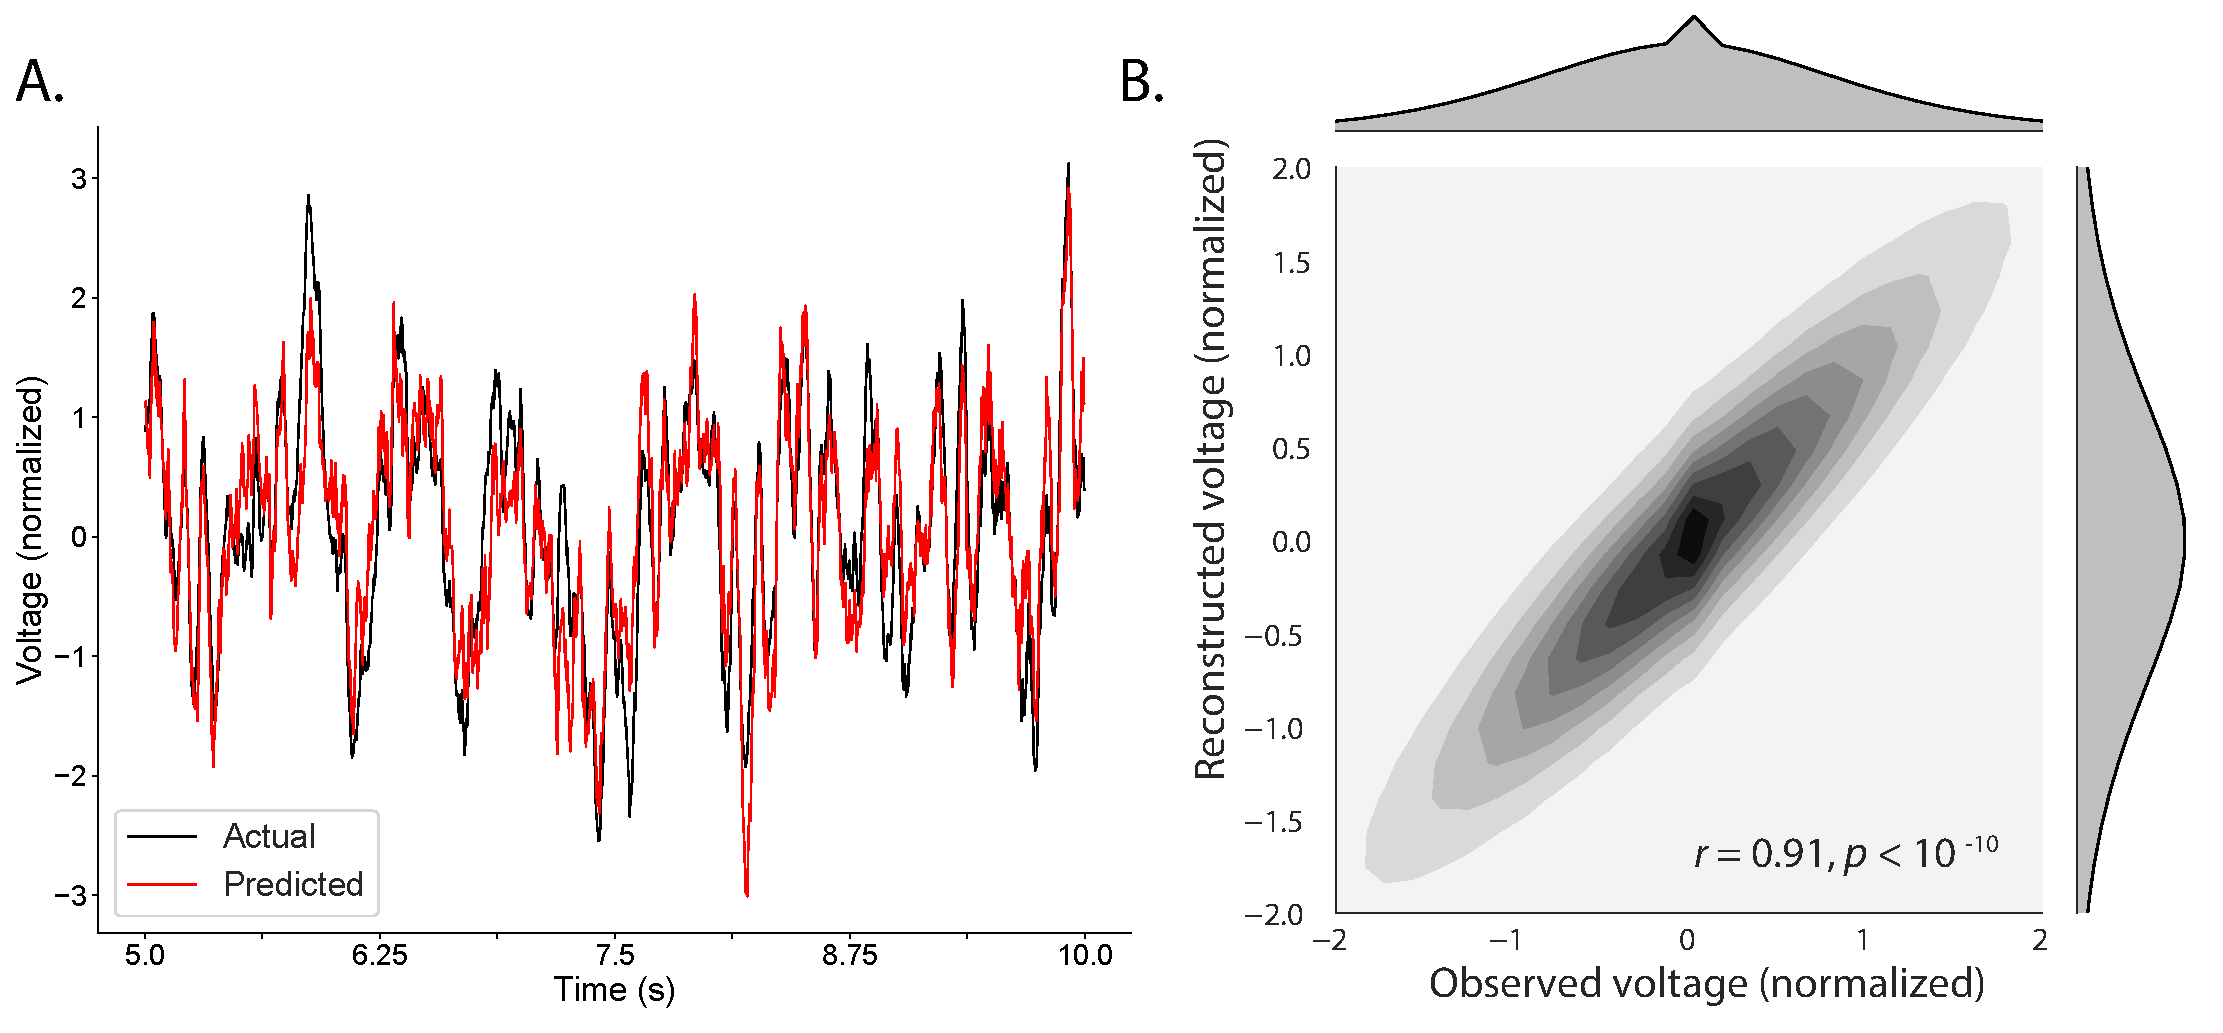
\includegraphics[width=\textwidth]{figs/recon}
  \caption{\textbf{Observed and reconstructed LFP from a single
      electrode.} \textbf{A. Example LFP.}  A 5~s recording from the
    red electrode in Figure~\ref{fig:methods}A is displayed in red,
    and the reconstructed LFP during the same time window is shown in
    blue.  \textbf{B. Observed versus reconstructed LFP over
      14.2~hours.}  The two-dimensional histogram reflects the
    relation between distributions of observed versus reconstructed
    voltages from one patient, across the 14.2 hours of recorded data
    collected over 6 recording sessions.  The correlation reported in
    the panel is between the observed and reconstructed voltages.
    Both panels: all voltages are represented in standard deviation units
   (computed within session).}
  \label{fig:recon}
\end{figure}

For each held-out electrode, from each held-out patient in turn, we we
computed the average correlation (across recording sessions) between
the SuperEEG-reconstructed voltage traces and the observed voltage
traces from that electrode.  For this analysis we set $\bar{R}$ to be
the union of all electrode locations across all patients.  This
yielded a single correlation coefficient for each electrode location
in $\bar{R}$, reflecting how well the SuperEEG algorithm was able to
recover the recording at that location by incorporating data across
patients (black histogram in Fig.~\ref{fig:corrmap}A, map in
Fig.~\ref{fig:corrmap}C).  The observed distribution of correlations
was centered well above zero (mean: XXX; $t$-test comparing mean of
distribution of $z$-transformed per-electrode correlation coefficients
to 0: $t(XXX) = XXX, p = XXX$), indicating that the SuperEEG algorithm
recovers held-out activity patterns substantially better than random
guessing.

As a stricter benchmark, we compared the quality of these
across-participant reconstructions (i.e., computed using a correlation
model derived from other patients' data) to reconstructions generated
using a correlation model trained using the in-patient's data.  In
other words, for this within-patient benchmark analysis we estimated
$\hat{C}_{s}$ (Eqn.~\ref{eqn:subj_corrmat}) for each patient in turn,
using recordings from all of that patient's electrodes except at the
location we were reconstructing.  These within-patient reconstructions
serve as an estimate of how well data from all of the other electrodes
from a single patient may be used to estimate held-out data.  This
allows us to ask how much information about the activity at a given
electrode might be inferred through (a) volume conductance or other
sources of ``leakage'' from activity patterns measured from the
patient's other electrodes and (b) across-electrode correlations
learned from that single patient.  As shown in
Figure~\ref{fig:corrmap}A (gray histogram), the distribution of
within-patient correlations was centered well above zero (mean: XXX;
$t$-test comparing mean of distribution of $z$-transformed
per-electrode correlation coefficients to 0: $t(XXX) = XXX, p = XXX$).
However, the across-patient correlations were substantially higher
($t$-test comparing average $z$-transformed within versus across
patient electrode correlations: $t(XXX) = XXX, p = XXX$).  This is an
especially conservative test, given that the across-patient SuperEEG
reconstructions exclude (from the correlation matrix estimates) all
data from the patient whose data is being reconstructed.  We repeated
each of these analyses on a second independent datset and found
similar results (Fig.~\ref{fig:corrmap}B, D; within versus across
reconstruction accuracy: $t(23) = 6.93, p < 10^{-5}$). Our finding,
that when reconstructing held-out data from a given patient
correlation models derived from \textit{other} patient's data yield
higher reconstruction accuracy than correlation models derived from
that patient, has two important implications.  First, it implies that
distant electrodes provide additional predictive power to the data
reconstructions beynd the information contained solely in nearby
electrodes.  (This follows from the fact that each patient's
electrodes are implanted in a unique set of locations, so for any
given electrode the closest electrodes in the full dataset are likely
to come from the same patient.)  Second, it implies that the spatial
correlations derived from the SuperEEG algorithm are, to some extent,
similar across people.

%correlations by brain area, distribution of correlations
\begin{figure}
  \centering
  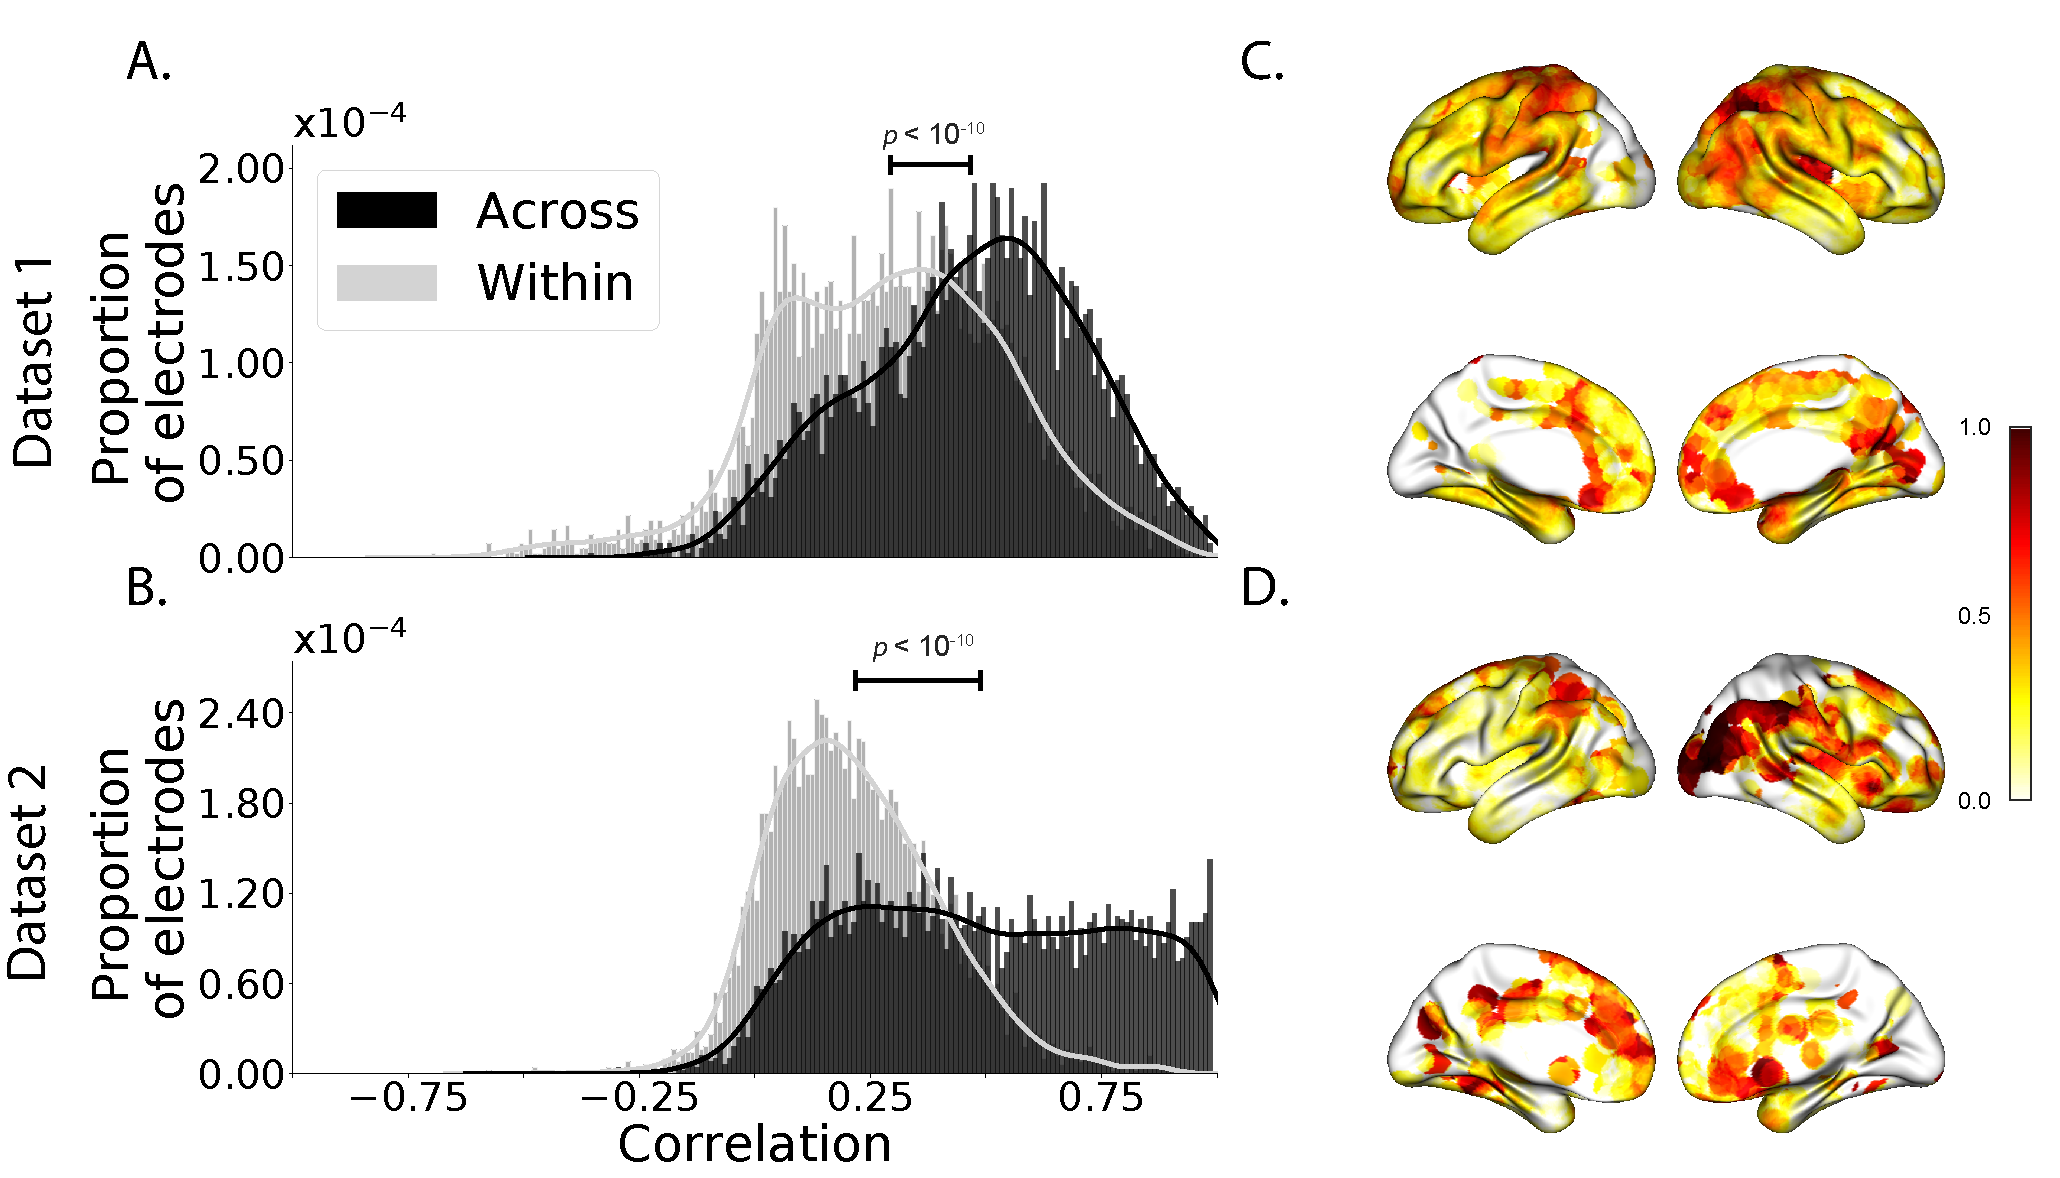
\includegraphics[width=\textwidth]{figs/corrmap}
  \caption{\textbf{Reconstruction quality across all electrodes in two
      ECoG datasets.}  \textbf{A. Distributions of correlations
      between observed versus reconstructed activity by electrode, for
      Dataset 1.}  The across-patient distribution (black) reflects
    reconstruction performance using a correlation model trained on
    all but one patient, and then applied to the held-out patient's
    data.  The within-patient distribution (gray) reflects performance using
    a correlation model trained on the same patient who contributed
    the to-be-reconstructed electrode.  \textbf{B. Distributions of
      correlations for Dataset 2.}  This panel is in the same format
    as Panel A, but reflects results obtained from Dataset 2.
    \textbf{C.--D.  Reconstruction performance by location.} Each dot
    reflects the location of a single implanted electrode from Dataset
    1 (Panel C) or Dataset 2 (Panel D).  The dot colors denote the
    average across-session correlation, using the across-patient
    correlation model, between the observed and
    reconstructed activity at the given electrode location.}
  \label{fig:corrmap}
\end{figure}

The recordings we analyzed from Dataset 1 comprised data collected as
the patients performed a variety of (essentially uncontrolled) tasks
throughout each day's recording session.  That we observed reliable
reconstruction accuracy across patients suggests that the spatial
correlations derived from the SuperEEG algorithm are, to some extent,
similar across tasks.  We tested this finding more explicitly using
Dataset 2.  In Dataset 2, the recordings were limited to times when
each patient was participating in each of two experiments (Experiment
1, a random-word list free recall task, and Experiment 2, a
categorized list free recall task).  We wondered whether a correlation
model trained using data only from one experiment might yield good
predictions for data from the other experiment.  Further, we wondered
about the extent to which it might be benefitial or harmful to combine
data across tasks.

\textbf{JRM STOPPED HERE}

We were interested in the task specific contributions to the
reconstruction accuracy.  Each patient in the the second dataset
participated in two free recall experiments.  We ran similar analyses
for both experiments and found that activity was best reconstructed
when limiting the training data to within task, as opposed to across
task or incorporating data from both tasks (Fig.~\taskrecon (mean reconstruction accuracy incorporating data within task: 0.55, across task: 0.37, all tasks: .50)). Although reconstruction accuracy in the across task analysis was still better than the volume conductance model alone (paired $t$-test
between $z$-transformed mean correlation coefficients by patient: $t(47) = 5.65, p < 10\textsuperscript{-5}$), these results suggests that having a common tasks for patients may yield better reconstruction accuracy.  

We also wondered whether reconstruction quality (measured as the
correlation between the observed and reconstructed data) varied with
the electrode locations (Fig.~\ref{fig:corrmap}B \& D). In general, reconstruction quality remained high throughout the brain. Although reconstruction accuracy appeared high in the medial temporal lobe, which is a common epileptic focus (and therefore a common target for electrode implantation), we observed a weak but statistically reliable negative correlation between reconstruction quality and electrode density (defined as the proportion of electrodes within 20 MNI units for each location; dataset 1: $r = -0.07, p < 10^{-5}$, dataset 2: $r = -0.16, p < 10^{-10}$). This provides some evidence that our reconstruction accuracy results cannot be driven only by volume conductance.  Qualitatively, it appeared that the distribution of electrodes was similar across the datasets, suggesting potential commonalities of target locations across patients and similarities in surgical decisions. Indeed, we found a relatively strong correlation between the electrode densities within the two datasets (defined as the proportion of electrodes within 20 MNI units for each 34686 voxels (Fig.~\ref{fig:density}A, B); $r = 0.57, p < 10^{-10}$).  



\begin{figure}
  \centering
  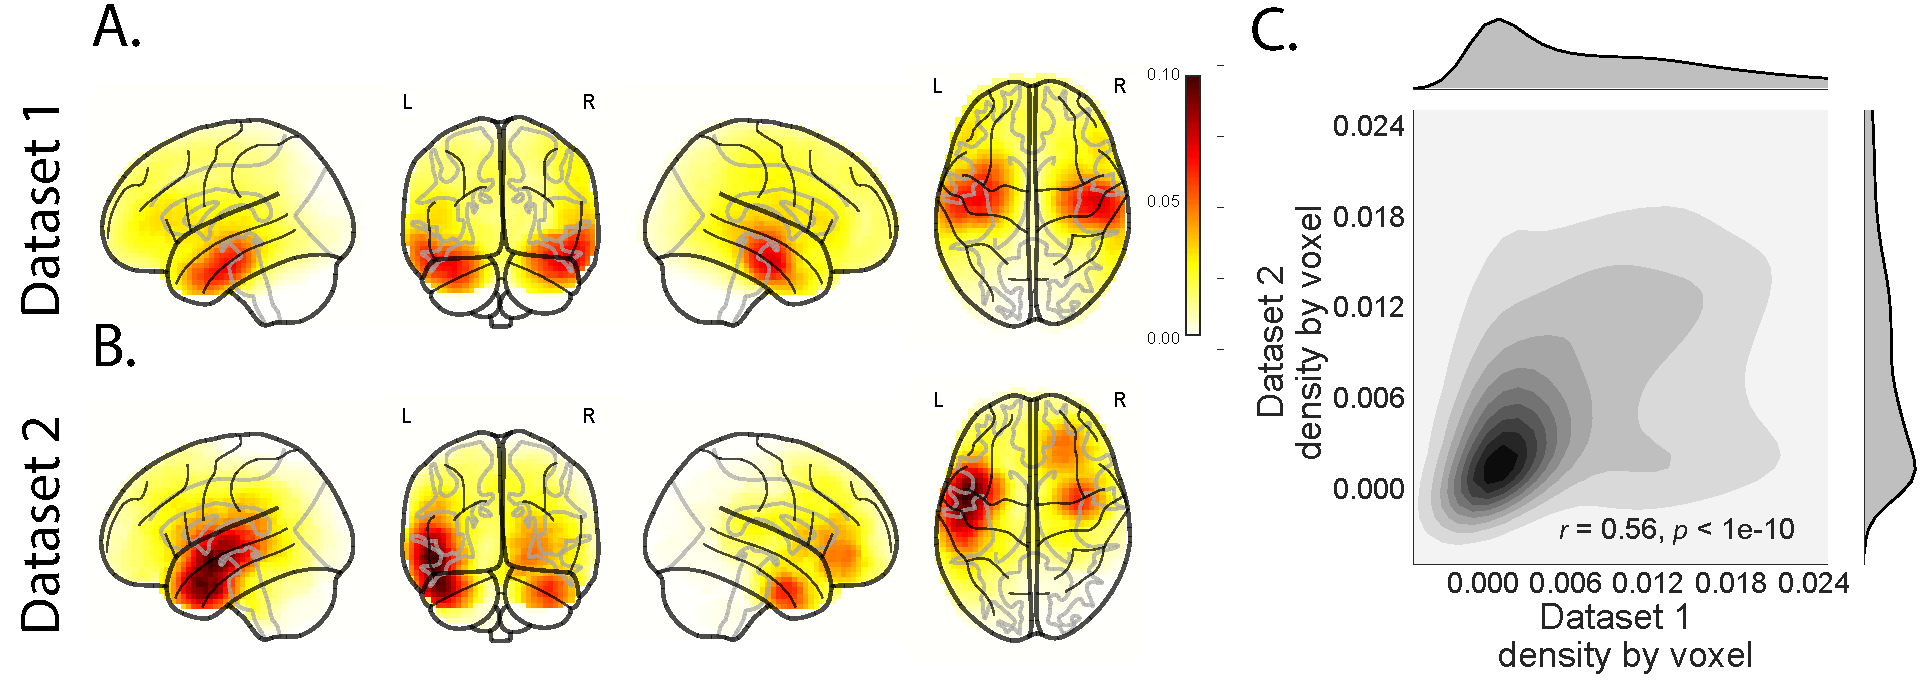
\includegraphics[width=\textwidth]{figs/density}
  \caption{\textbf{Sampling density and reconstruction quality.}
    \textbf{A. \& B. } The glass brain maps show sampling density by voxel location for dataset 1 and dataset 2. \textbf{C.}
      Correlation of sampling density by voxel location for dataset 1 vs. dataset 2.}
  \label{fig:density}
\end{figure}

In addition to exploring how reconstruction quality varies with
location, we also wondered whether there might be effects of electrode
placements on reconstruction quality.  For example, are there
particular implantation locations that yield especially high
reconstruction accuracies at other locations throughout the brain? To gain insights into this questions, we computed the average reconstruction correlation for each patient, then computed the average patient reconstruction correlation for any patients who had electrodes within a 20 MNI unit diameter sphere centered on each voxel location. The resulting maps highlight the locations of implanted electrodes from patients whose
reconstructions were especially accurate  (Fig.~\ref{fig:informap}A and B). We found that the most informative locations were consistent across datasets which lends support to the notion that different electrode location are more informative about activity across patients (Fig.~\ref{fig:informap}C); $r = 0.22, p < 10^{-10}$).  The locations in dark red might therefore be good candidate
implantation targets for neurosurgeons and neurologists who wish to
use SuperEEG to reconstruct full-brain electrophysiological signals.
The above findings, that one can infer brain activity throughout a person's brain 
using recordings from a limited number of locations from that person's brain in conjunction with recordings from other people's brains, have deep
implications for the structure of brain data.  The first implication
is that the correlational structure of different people's brain data
is largely preserved across individuals. Despite recent evidence that different people have stable but reliably different resting state connectome~\cite{FinnEtal15}, our results suggest that the correlational structure of different people's brain data is preserved enough across individuals to provide meaningful information. 

\begin{figure}
  \centering
  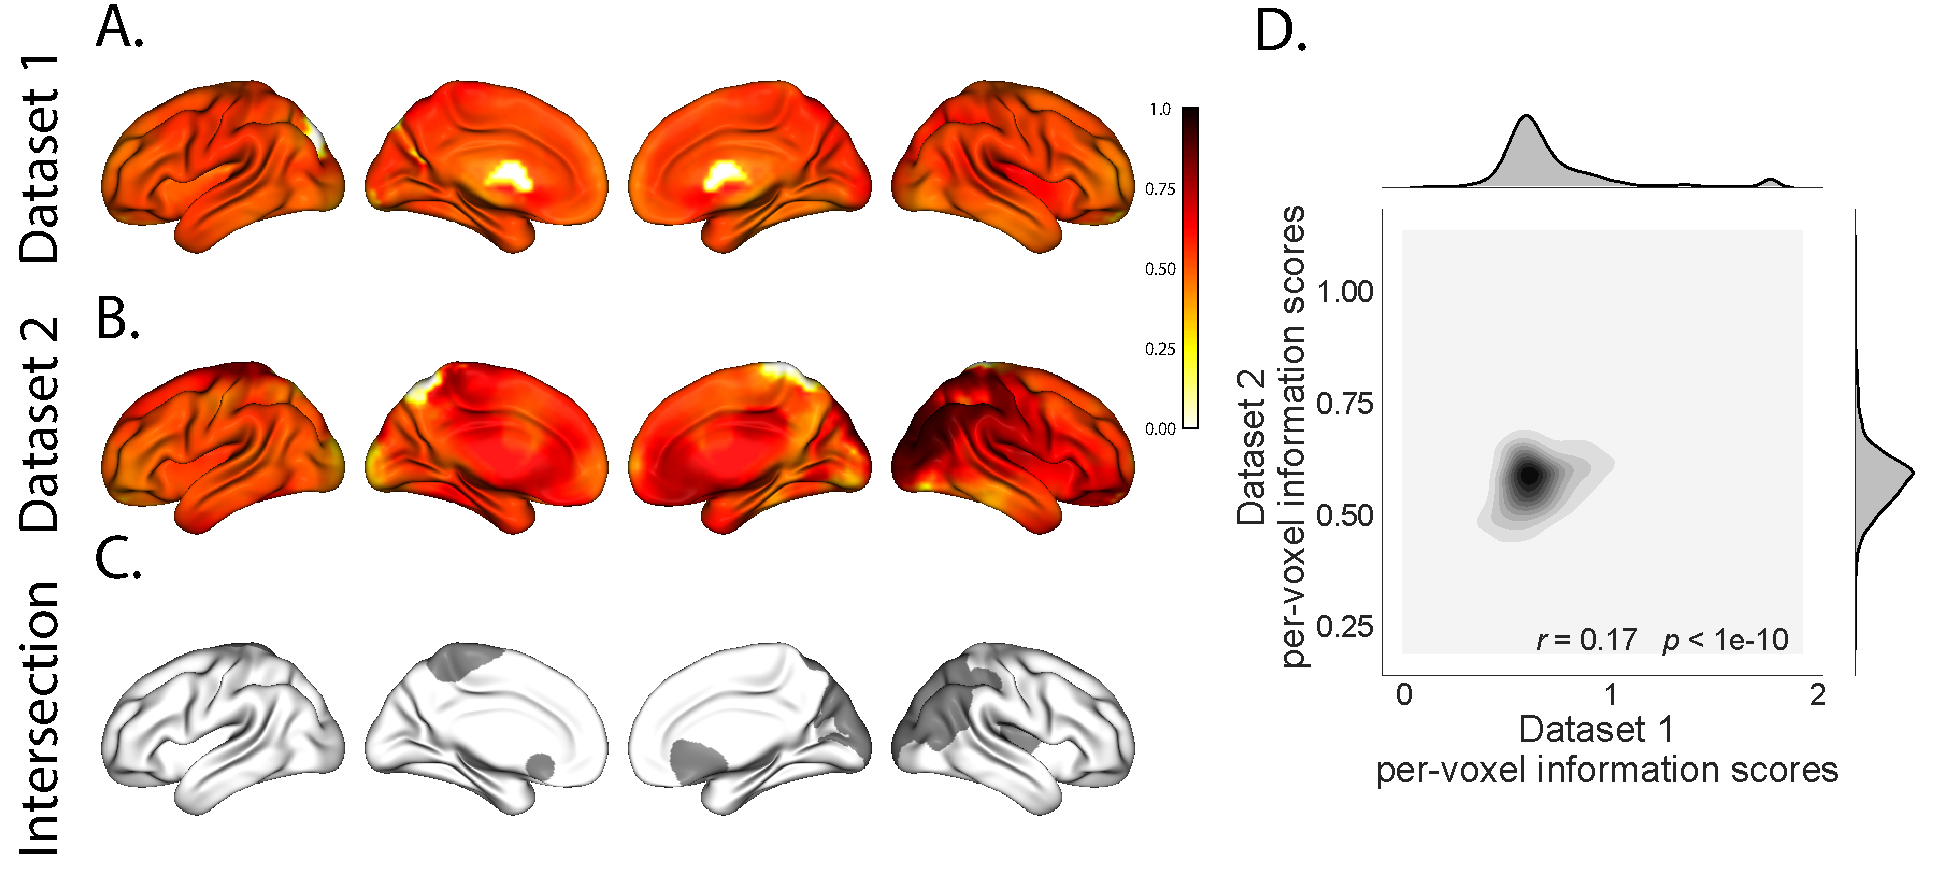
\includegraphics[width=\textwidth]{figs/informap}
  \caption{\textbf{Most informative electrode locations.} \textbf{A. \& B. } The glass
    brain maps displays the average reconstruction correlations (by patient, across
    all electrodes) for patients with electrodes within a 20 MNI unit diameter sphere centered on
    each location for dataset 1 and dataset 2. \textbf{C.} Correlation between z-transformed correlations by voxel for dataset 1 vs. dataset 2.}
  \label{fig:informap}
\end{figure}


\section*{Discussion}
%DISCUSSION POINTS
%recap main approach
SuperEEG infers full-brain activity patterns by leveraging
correlations in those patterns of brain activity within and across people.  Although
the approach may, in principle, be used to infer brain activity
\textit{anywhere} in the brain, the inferences perform slightly better for
regions with dense electrode sampling across patients.  (Taken to the logical extreme, we could not hope to accurately recover activity patterns from brain areas where no recordings existed from any patient.)   As more data
are included in the inference procedure, this suggests that reconstruction accuracy should improve.

%why does it work?  redundancy of brain
A fundamental assumption of the SuperEEG algorithm is that the data
covariance matrix is stable over time and across people.  This is a
useful simplification.  However, a growing body of evidence from the
fMRI community suggests that the data covariance matrix changes in
meaningful ways over time (for example, the data covariance matrix
changes from moment-to-moment during story listening, serving as a
unique ``fingerprint'' for each moment of the story; further, these
task-driven timepoint-specific covariance fingerprints appear to be
largely preserved across people~\cite{SimoEtal16, MannEtal17}).  These
findings indicate that the full-brain covariance matrix is not stable
over time.  Other recent work has shown that people's resting state
connectivity matrices may be used to uniquely identify individuals and
predict fluid intelligence scores~\cite{FinnEtal15}.  This indicates
that the full-brain covariance matrix is not stable across people.  If
the fundamental stability assumptions that SuperEEG relies on are
violated, how can the SuperEEG algorithm still accurately recover LFP
data?  It is important to recognize that the fact that variability
(over time or across people) is predictive (e.g., of cognitive states
during story listening or fluid intelligence scores) does not
necessarily mean that this variability is large in magnitude.  Rather,
we have long known that brain structure is tightly preserved across
individuals (and over time, at least on the timescale of typical
clinical and experimental recording sessions), and any functional
changes must occur within the framework of the underlying structural
anatomy.  Nevertheless, one could imagine future improvements to the
SuperEEG approach that leverage resting state fMRI or structural data
[e.g., diffusion tensor imaging (DTI)] to estimate Bayesian priors over
the correlation matrices inferred, in the current framing, using only
ECoG data.  Further, relaxing the assumption that the covariance
matrix is stable (over time and/or across people), and/or
incorporating more detailed brain conductance models (e.g., informed
by structural MRI scans) may improve the predictive performance of the
approach.



%This technique relies on recordings from many patients performing the
%same basic cognitive task.  To what extent do these findings
%generalize across studies?  For example, could one combine recordings
%from several studies to improve our ability to reconstruct neural
%activity?
One potential limitation of the SuperEEG approach is that the above
assumption of covariance stability across people may be violated even
more if different patients are performing different cognitive tasks.
To understand of the extent to which the current findings generalize across
cognitive tasks, we replicated our initial findings using a dataset in which patients participated in two tasks, and limited the training data to either within task, across task, or using both tasks. Since we found the most accurate reconstructions using task-specific data, this would suggest building up new databases for estimating each task-specific covariance
matrix.  Or, using a more sophisticated approach, one could create a
hierarchical model whereby each task-specific covariance matrix was
modeled as a perturbation of a ``global'' task-unspecific covariance
matrix (which could in turn be informed by fMRI or DTI data).
% Alternatively, if the covariance matrix is stable across tasks, this would
% suggest that recordings from multiple studies could be combined to
% improve the overall reconstruction accuracy.

A second potential limitation of the SuperEEG approach is that it
does not provide a natural means of estimating the precise timing of
single-neuron action potentials.  Prior work has shown that gamma band
and broadband activity in the LFP may be used to estimate the firing
rates of neurons that underly the population contributing to the
LFP~\cite{MannEtal09}.  Because SuperEEG reconstructs LFPs throughout
the brain, one could in principle use gamma or broadband power in the
reconstructed signals to estimate the corresponding firing rates
(though not the timings of individual action potentials).

Beyond providing a means of estimating ongoing activity throughout the
brain using already implanted electrodes, our work also has
implications for where to place the electrodes in the first place.
Electrodes are typically implanted to maximize coverage of suspected
epileptogenic tissue.  However, our findings suggest that this approach
could be further optimized.  Specifically, one could leverage not only
the non-invasive recordings taken during an initial monitoring period
(as is currently done), but also recordings collected from other
patients.  We could then ask: given everything we know about the other
patients and from the scalp recordings of this new patient, where
should we place a fixed number of electrodes to maximize our ability
to map seizure foci?  As shown in Figure~\ref{fig:informap}, recordings
from different locations are differently informative in terms of
reconstructing the spatiotemporal patterns throughout the brain.
This property might be leveraged in decisions about where to
surgically implant electrodes in future patients.


\section*{Concluding remarks}
Over the past several decades, neuroscientists have begun to leverage
the strikingly profound mathematical structure underlying the brain's
complexity to infer how our brains carry out computations to support
our thoughts, actions, and physiological processes.  Whereas
traditional beamforming techniques rely on geometric
source-localization of signals measured at the scalp, here we propose
an alternative approach that leverages the rich correlational
structure of a large dataset of human intracranial recordings.  In
doing so, we are one step closer to observing, and perhaps
someday understanding, the full spatiotemporal structure of human
neural activity.

\section*{Code availability}
We have released an open-source SuperEEG Python toolbox.  All of the code used in this manuscript is on GitHub, and the code may be shared using a GitHub account accessible to the reviewers upon request.

\section*{Data availability}
The dataset analyzed in this study was generously shared by Michael J. Kahana.  A portion of the dataset may be downloaded \href{http://memory.psych.upenn.edu/Request_EEG_access?paper=SedeEtal03}{\underline{here}}.
\section*{Acknowledgements}
We are grateful for useful discussions with Luke J. Chang and Matthijs van der Meer.  We are also grateful to Michael J. Kahana for generously sharing
the ECoG dataset we analyzed in our paper, which was collected under
NIMH grant MH55687 to MJK.  Our work was also supported in part by NSF EPSCoR Award Number 1632738.  The content is solely the responsibility of the authors and does not necessarily represent the official views of our supporting organizations.
\section*{Author Contributions}
J.R.M conceived and initiated the project. L.L.W.O. and A.C.H. performed the analyses. J.R.M. and L.L.W.O. wrote the manuscript.

\section*{Author Information}
Reprints and permissions information is available at www.nature.com/reprints.  The authors declare no competing financial interests.  Readers are welcome to comment on the online version of the paper.  Publisher's note: Springer Nature remains neutral with regard to jurisdictional claims in published maps and institutional affiliations.  Correspondence and requests for materials should be addressed to J.R.M.  (jeremy.r.manning@dartmouth.edu).

\bibliography{CDL-bibliography/memlab.bib}
\bibliographystyle{Science}

\clearpage

\end{document}




















